\subsection{The straightforward approach}
\label{chap:straightforward_approach}

The first attempt was quite straightforward and a little bit explorative, in the way, that the author had to discover the MPS API, that allows programmatical language generation.
Because MPS is still in development, the API isn't that well documented and some features had to be discovered through trial and error or through examination of the PE4MPS project (\ref{chap:pe4mps}), which served great aid here.

\subsubsection{The algorithm}
\label{chap:straight_algorithm}
The main idea behind the first attempt comes from the realization, that when a parser rules breaks into more alternatives, we need to create a concept for each alternative.
Then we have to somehow mark them as belonging to that parser rule.
Consider the \parserrule{content} rule from our SimpleXML language:

\begin{antlr}
	\parserrule{content}    :   \lexerrule{TEXT}
           |   \parserrule{element}
           |   \parserrule{comment}
           |   \lexerrule{CDATA}
           ;
\end{antlr}

We will need to have 4 concepts, that could appear anywhere the \parserrule{content} rule is referenced.
That is why we decided, that for each rule with more than one alternative, we will create an interface concept.
Then for each alternative of this rule, we will create a concept, that will implement this interface.
So for our \parserrule{content} example, we will get following setup:

\begin{antlr}
	\interface{IContent}   :   \concept{Content{\_}1}
           |   \concept{Content{\_}2}
           |   \concept{Content{\_}3}
           |   \concept{Content{\_}4}
\end{antlr}

Names of these concepts are derived from the name of the rule, numbers are added to alternatives correspondingly.
For rules with a single alternative, no interface is needed.
For rules, that contain in-line block rules (\ref{chap:subrules}), we have already created artificial parser rules in our tree representation during the parser phase (\ref{chap:parsing_the_grammar}), which means we do not have to worry about them now.
\\

Now we will describe, how we linked parser rules together.
Consider the \parserrule{element} rule, that is referencing the \parserrule{content} rule:

\begin{antlr}
	\parserrule{element}    :   \literal{<} \lexerrule{Name} \parserrule{attribute}* \literal{>} \parserrule{content}* \literal{</} \lexerrule{Name} \literal{>}
           |   \literal{<} \lexerrule{Name} \parserrule{attribute}* \literal{/>}
           ;
\end{antlr}

Following the algorithm mentioned above, there is one \interface{IElement} interface and two \concept{Element{\_}1}, \concept{Element{\_}2} concepts created.
For each referenced parser rule inside a concept, we create a child link and point it to the right interface.
In our example, for concept \concept{Element{\_}1}, there would be two child links pointing to \interface{IAttribute} and \interface{IContent}.
In figure \ref{fig:element_concept_full}, you can see the full \concept{Element{\_}1} concept.

\begin{figure}[h]
	\centering
	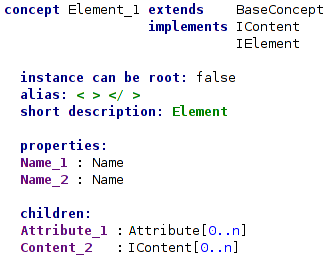
\includegraphics[scale=0.7]{./img/element_concept_full.png}
	\caption{Element{\_}1 concept's structure aspect}
	\label{fig:element_concept_full}
\end{figure}

Naming convention of child links also contains numbers, because names have to be unique.

\subsubsection{The layer problem}
\label{chap:layer_problem}

The algorithm mentioned above will leave us with an MPS language, that follows given structure correctly and could be used to represent code in that language inside MPS correctly. Editing the code will not be possible yet, as there is no editor aspect defined so far.
There is one problem, however, concerning usability of such language.
We will demonstrate this problem on the SimpleXML language, using \parserrule{element} and \parserrule{content} rules:

\begin{antlr}
	\parserrule{content}    :   \lexerrule{TEXT}
           |   \parserrule{element}
           |   \parserrule{comment}
           |   \lexerrule{CDATA}
           ;

	\parserrule{element}    :   \literal{<} \lexerrule{Name} \parserrule{attribute}* \literal{>} \parserrule{content}* \literal{</} \lexerrule{Name} \literal{>}
           |   \literal{<} \lexerrule{Name} \parserrule{attribute}* \literal{/>}
           ;
\end{antlr}

When we would be editing code in this language, the MPS auto-complete would give us aid when filling out all properties and children of inserted concepts.
Imagine there is a freshly inserted \concept{Element{\_}1} concept (a concept representing the full XML element as is stated in the first alternative of the \parserrule{element} parser rule).
This setup can be seen in the left part of figure \ref{fig:layer_problem}.
Now, we would like to insert some content inside.
Let's say we would like to insert a nested XML element inside.
We would place cursor in the content placeholder and press Ctrl+Space to view the auto-completion options.
\\

Following the algorithm mentioned above, we have created a child link of the \concept{Element{\_}1} concept of type \interface{IContent}.
There exist 4 concepts, that implement the \interface{IContent} interface as per each alternative of the rule.
MPS evaluates this and gives us 4 options inside the auto-complete.
This auto-complete is captured in figure \ref{fig:layer_problem}.

\begin{figure}[h]
	\centering
	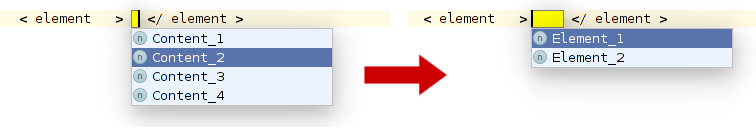
\includegraphics[width=\textwidth]{./img/layer_problem.png}
	\caption{Layer problem in auto-completion}
	\label{fig:layer_problem}
\end{figure}

In order to correctly insert another nested element inside, we would have to first insert a \concept{Content{\_}2} concept inside \concept{Element{\_}1}, that has an \interface{IElement} child inside (and nothing else).
Then, as a second step, we would call for the auto-complete again and insert either \concept{Element{\_}1} or \concept{Element{\_}2} inside \concept{Content{\_}2}.
This mean that we have to go through two steps and in the first one either guess correctly (or remember the grammar rule's alternative order), to know, which item of the auto-complete we should go with.
\\

And the problem goes both ways --- if we decide to replace the nested \concept{Element{\_}1} with, let's say, an XML comment (a \concept{Comment} concept), we need to delete both intermediary layers before we get back to the original \concept{Content{\_}X} crossroads.
Meanwhile the user cannot really see, what is happening, since the intermediary level has no appearance or indicator.
This leads to confusion on user's part.
\\

We tried to ease this situation up by creating aliases for concepts derived from their content (names such as “Element content” or “CDATA content” instead of Content{\_}N), but the problem goes beyond this.
Take into consideration, that the SimpleXML grammar is a very simple one.
More sophisticated languages may have more than two intermediary layers and writing code would consist of clicking through a large number of auto-completes like shown in the example above.
There is also nothing preventing authors of grammars from naming these helper layers in a completely unrelated manner, which would make user's orientation even harder.
After all, these layers come into existence when the grammar is being written, so that it is more readable for humans and maybe better maintainable by the author.
It has nothing to do with making the AST simple for the ANTLR parser.
ANTLR is very capable and handles this probably very well in any form.
\\

Furthermore, using in-line subrule blocks makes this even a bigger problem as the block rule's names are auto-generated by our parser and differ only by numbers, even though the alias assigning process improves the situation by a bit.
But from the point of view of the grammar's author, it is an invisible layer of rules nested inside.
\\

For better illustration, we have put examples of languages, that were generated by this algorithm, on the attached DVD. The reader can try them out on their own and see for themselves that this makes the language very unfriendly and hard to use. [TODO: DVD location]
